\documentclass[english,onecolumn]{IEEEtran}
\IEEEoverridecommandlockouts
\usepackage[T1]{fontenc}
%\usepackage[latin9]{luainputenc}
\usepackage[letterpaper]{geometry}
\geometry{verbose}
\usepackage{amsfonts}
\usepackage{babel}

\usepackage{extarrows}
\usepackage[colorlinks]{hyperref}
\usepackage{listings}
\usepackage{xcolor}
% \usepackage[ruled,linesnumbered]{algorithm2e}
\usepackage{longtable}
\usepackage{amsmath,graphicx}
\usepackage{subfigure} 
\usepackage{cite}
\usepackage{amsthm,amssymb,amsfonts}
\usepackage{textcomp}
\usepackage{bm}
\usepackage{booktabs}
\usepackage{listings}
\definecolor{salmon}{rgb}{1, 0.5020, 0.4471}
\usepackage{xparse}



\usepackage[noend]{algpseudocode}
\usepackage{algorithmicx,algorithm}

\NewDocumentCommand{\codeword}{v}{%
\texttt{\textcolor{blue}{#1}}%
}

\lstdefinestyle{mystyle}{
    numberstyle=\color{green},
    numbers=left,                    
    numbersep=5pt,                  
    showspaces=false,                
    showstringspaces=false,
    showtabs=false,                  
    tabsize=2
}

\lstset{style=mystyle}

\providecommand{\U}[1]{\protect\rule{.1in}{.1in}}
\topmargin            -18.0mm
\textheight           226.0mm
\oddsidemargin      -4.0mm
\textwidth            166.0mm
\def\baselinestretch{1.5}


\newcommand{\Rbb}{\mathbf{R}}
\newcommand{\Pb}{\mathbf{P}}
\newcommand{\Ib}{\mathbf{I}}
\newcommand{\vb}{\mathbf{v}}
\newcommand{\Ucal}{\mathcal{U}}
\newcommand{\Wcal}{\mathcal{W}}
\newcommand{\Vcal}{\mathcal{V}}
\newcommand{\Rcal}{\mathcal{R}}
\newcommand{\Ncal}{\mathcal{N}} 


\def\Q{\mathbf{Q}}
\def\A{\mathbf{A}}
\def\U{\mathbf{U}}
\def\R{\mathbf{R}}
\def\I{\mathbf{I}}

\def\a{\mathbb{a}}



%\begin{abstract}
%This document is a model and instructions for \LaTeX.
%This and the IEEEtran.cls file define the components of your paper [title, text, heads, etc.]. *CRITICAL: Do Not Use Symbols, Special Characters, Footnotes, 
%or Math in Paper Title or Abstract.
%\end{abstract}

%\begin{IEEEkeywords}
%component, formatting, style, styling, insert
%\end{IEEEkeywords}


\begin{document}
	
	\title{NMF-GNN: Full Global Structure Enhancement of Structural-sensitive Message Passing in Graph Neural Networks*\\

		\thanks{Identify applicable funding agency here. If none, delete this.}
	}
	
	\author{
		\IEEEauthorblockN{Xinnan Dai}\\
		\IEEEauthorblockA{\textit{School of Information Science and Technology} \\
			\textit{ShanghaiTech University}\\
			Shanghai, China\\
			201210}\\
		\and
		\IEEEauthorblockN{Chenyu He}\\
		\IEEEauthorblockA{\textit{School of Information Science and Technology} \\
		\textit{ShanghaiTech University}\\
		Shanghai, China\\
		201210}
		%\and
		%\IEEEauthorblockN{3\textsuperscript{rd} Given Name Surname}
		%\IEEEauthorblockA{\textit{dept. name of organization (of Aff.)} \\
		%\textit{name of organization (of Aff.)}\\
		%City, Country \\
		%email address or ORCID}
		%\and
		%\IEEEauthorblockN{4\textsuperscript{th} Given Name Surname}
		%\IEEEauthorblockA{\textit{dept. name of organization (of Aff.)} \\
		%\textit{name of organization (of Aff.)}\\
		%City, Country \\
		%email address or ORCID}
		%\and
		%\IEEEauthorblockN{5\textsuperscript{th} Given Name Surname}
		%\IEEEauthorblockA{\textit{dept. name of organization (of Aff.)} \\
		%\textit{name of organization (of Aff.)}\\
		%City, Country \\
		%email address or ORCID}
		%\and\usepackage[noend]{algpseudocode}
		%\IEEEauthorblockN{6\textsuperscript{th} Given Name Surname}
		%\IEEEauthorblockA{\textit{dept. name of organization (of Aff.)} \\
		%\textit{name of organization (of Aff.)}\\
		%City, Country \\
		%email address or ORCID}
	}
	
	\maketitle
	
	
	
	
	
	\section{Introduction}
	\subsection{Current work}
	Currently typical message passing mechanisms of graph neural networks (GNN) are highly related to the graph structure. For example, graph attention networks (GAT)\cite{gat} passes information via attention sharing on global nodes, graph convolution network (GCN)\cite{gcn} performs Laplacian approximations on spectral convolution. More specifically, message passing process of GCN follows the eigenvalue and eigenvector of Laplacian matrix, which is strong structure-related. However, there still exists information which are not position-aware, which indicates they are unable to be shared during the position aware message passing. For example, in relation networks like social networks and citation networks, there may exists orphan nodes which contains features not similar to those of connected nodes. Typical solution is random sampling on the whole node set of the graph, regardless of the edge connections. Thus successful extraction of these structure-independent features may significantly boosts the representation performance of the node. Typical solution is random sampling on the whole node set of the graph, regardless of the edge connections. For example, P-GNN\cite{b1} randomly samples several subsets containing arbitrary count of nodes on the original graph, and stacks as a  feature matrix. All subsets further aggregate into a shared vector by aggregation (subset-wise mean), and fused to each node feature vector. While GraphSTONE\cite{b2} divides the graph via random walk and find shared information from different samples on the unique structure topic. However, random sampling cannot perfectly extract the global information, which performance may influenced by the randomly sampled result. Mechanics with direct operation on the whole graph is required. 
	
	Non-negative matrix factorization (NMF) is a matrix factorization mechanism which is able to learn parts-based representations by 2 low rank matrices, as the linear combination of the data-based basis and weights \cite{b3}, like other typical factorization methods like principle component analysis (PCA) and vector quantization (VQ). Among which, eigen-based methods PCA and VQ mainly extracts holistic features, where basis components manifesting building blocks of the original matrix may missing \cite{b4}. 
	NMF makes the computation more efficient and has achieved wide application in engineering, such as data mining and image processing, to name a few. In image processing, \cite{b3} and \cite{b4} uses NMF to calculate the basis representation of human face data in facial recognition and classification tasks. In data mining, NMF is able to calculate the semantic feature representations in articles\cite{b3}. NMF has also become a basic baseline algorithm in recommendation system as representing the individual-item relation by refined individual-topic and topic-item relations. Besides, GraphSTONE\cite{b2} also uses NMF to factorize the key structure topic of sampled results from different random walks, and lead to the following principal component calculation. However typically, NMF is applied in end to end approaches as feature extractor,  where potential distribution shift may exists between the learned representation by NMF and the original node features. Thus separated implement of NMF may still cause performance decreasing in contrast with the approach without NMF. 
	
	\subsection{Our contribution}
	We purpose a novel approach enhancing the message passing of GNNs via non-negative matrix factorization (NMF), for leading the structure-invariant components into the node features. Inspired by above researches, we directly perform NMF on the feature matrix and gained a global basis matrix and the corresponding weight matrix. The operation on the whole matrix imposes the global feature distribution into the factorized basis, which is further embedded into a feature vector and send into message passing together with original node features. 
	Furthermore, to better integrate NMF into message passing framework,  the basis matrix is randomly initialized and update via backward propagation with the whole graph rather than explicitly perform NMF on the original feature matrix, to achieve distribution consistency between the feature of basis representation and node features. 
	
	\section{Methods}
	
		\subsection{Non-negative matrix factorization}
	Non-negative matrix factorization (NMF) is a matrix factorization method wildly used in recommend systems and text mining. In the text mining task, we use this method to analyze text topics. For any text sets with $n$ texts and $m$ words, given an nonnegative matrix $\mathbf{X}\in\mathbb{R}^{n\times m}$, it can find a nonnegative matrix $\mathbf{W}\in\mathbb{R}^{n\times t}$ to represent the relevance of each text to $t$ topics, and a nonnegative matrix $\mathbf{H}\in\mathbb{R}^{t \times m}$ to show how the topics relate to the words, which satisfies the condition $\bf X=WH$, and decomposes a nonnegative matrix into the product of left and right nonnegative matrices. The text $\bf X$ is restructured by $\bf W$ and $\bf H$, consequently, the goal is $\bf min||X-WH||^2$. The update rule for NMF algorithm is in Algorithm 1 according to \cite{nips}.
	
	\begin{algorithm}[t]
		\caption{NMF} %算法的名字
		\hspace*{0.02in} { Input: $X$, max iteration number $iter$} %算法的输入, \hspace*{0.02in}用来控制位置,同时利用 \\ 进行换行
		\hspace*{0.02in} {\bf Output: $W,H$} %算法的结果输出
		\label{NMF}
		\begin{algorithmic}[1]
			\State random initial $W$ matrix and $H$ matrix % \State 后写一般语句
			\For{$i$ in $iter$} % For 语句,需要和EndFor对应
			\State  $H'\leftarrow H \frac{W^TX}{W^TWH}$
			\State $W'\leftarrow W\frac{XH^T}{WHH^T}$
			\State $H\leftarrow H'$
			\State $W\leftarrow W'$
			\EndFor
			\Return $W,H$
		\end{algorithmic}
	\end{algorithm}
	\subsection{Spatial Graph}
	Graph neural network is a method of connecting information between samples. This method can predict the information of neighbor nodes according to the properties of the points. Among them, most graph networks are based on spectral graph theory. A graph is defined as $G=(X,E)$, where $X=\{\bf x_1,x_2,\dots,x_n\}$ is the node set and $\bf E\in\mathbb{R}^{n\times n}$ represent whether exist the edges in the graph. To simulation the fusion on the graph, we use the Laplacian matrix which is $\bf L=D-E=dI-E=U\Lambda U^T$, where $\bf U$ is eigenvector matrix and $\bf \Lambda$ is the eigenvalue diagonal matrix. According to the definition of the matrix, the motion direction of the vector can be changed by the matrix $A$. For each vector in the graph, the transition is $\bf \lambda x =A x$.\cite{2} In the Laplacian transmition,  $A\in\mathbb{R}^{n\times n}$ is an approximate matrix based on Chebyshev Theory and $\theta\in\mathbb{R}^{n\times n}$. Thus, the transition is
	\[
	\bf g_{\theta}x=Ug_{\theta}U^Tx=Ug_{\theta}(\Lambda)U^Tx=Ax,
	\]
	where $\bf g_{\theta}$ is the a diagonal matrix with Chebyshev characteristic of $\lambda$, and $\bf g_{\theta}=g_{\theta}(\Lambda)$\cite{3}. Thus, the Laplasian transition is in the Chebyshev form where $\bf \tilde{L}=U\tilde{L}U^T, \tilde{L}=A$ and since the $\bf g_{\theta}x=Ax=\tilde{L}x$. In GCN \cite{gcn}, the transition is approximate to,
	\[
	\bf g_{\theta}x=\theta_0x-\theta_1D^{-1/2}ED^{-1/2}x.
	\]
	For simplicity, supposing $\theta=\theta_0=-\theta_1$, the form is,
	\[
	\bf g_{\theta}x=\theta(I+1D^{-1/2}ED^{-1/2})x.
	\]
	After the normalization,
	\[
	\bf \hat{X}=\tilde{D}^{-1/2}E\tilde{D}^{-1/2}\Theta X,
	\]
	where $\bf \Theta\in\mathbb{R}^{n\times m}$.
	
	As shown below, the GCN describ the information transition based on the edges. Similarly, the graph attention network (GAT) is in the form of $\bf \hat{X}=EW_bX$, where $\bf W_b$ is the weight matrix from attention coefficient\cite{gat}. Both GCN and GAT defines the information transition through the edges with the information from neigbor nodes. However, the labels also depend on the similar contents among the whole dataset.
	
	%Non-negative matrix factorization (NMF) is a matrix approximation mechanism of representing the big original matrix $ A $ by the product of 2 low rank matrices as $ \bf A\approx WH $. Among which, the factorization can be represented as expressing the original matrix by a set of more related basis, where $ \bf W $ is the basis matrix and $ \mathbf{H} $ is the projection to those basis.
	
	%\section{Results}
	%We've implemented a naive run on Cora dataset\cite{cora}, which consists 2708 scientific publication instances classified into 7 classes. The dataset provides a publication-keywords-classification characteristic table and a publication-publication citation relationship table. The implementation uses mean method to aggregate basis matrix into global feature vector, and uses GAT as the message passing backbone. The experiment result is shown in table \ref{result}, where the model is run on single NVIDIA GTX 1080 Ti GPU. Current implement has become a effective approximate of original GAT, while still exists optimization. 
	%
	%\begin{table}[htbp]
	%	\caption{Performances of our implementation compared to original GAT, measured in ROC AUC.}
	%	\begin{center}
	%	\begin{tabular}{|c|c|c|}
	%		\hline
	%		Implements & Inference Accuracy & Time consultant on each epoch (s) \\
	%		\hline
	%		GAT& 0.8453 & 0.912s \\
	%		\hline
	%		Ours& 0.8167 & 1.108s \\
	%		\hline
	%	\end{tabular}
	%	\label{result}
	%	\end{center}
	%\end{table}
	
	%\section*{Acknowledgment}
	%
	%The preferred spelling of the word ``acknowledgment'' in America is without 
	%an ``e'' after the ``g''. Avoid the stilted expression ``one of us (R. B. 
	%G.) thanks $\ldots$''. Instead, try ``R. B. G. thanks$\ldots$''. Put sponsor 
	%acknowledgments in the unnumbered footnote on the first page.
	
	%\section*{References}
	
	%Please number citations consecutively within brackets \cite{b1}. The 
	%sentence punctuation follows the bracket \cite{b2}. Refer simply to the reference 
	%number, as in \cite{b3}---do not use ``Ref. \cite{b3}'' or ``reference \cite{b3}'' except at 
	%the beginning of a sentence: ``Reference \cite{b3} was the first $\ldots$''
	%
	%Number footnotes separately in superscripts. Place the actual footnote at 
	%the bottom of the column in which it was cited. Do not put footnotes in the 
	%abstract or reference list. Use letters for table footnotes.
	%
	%Unless there are six authors or more give all authors' names; do not use 
	%``et al.''. Papers that have not been published, even if they have been 
	%submitted for publication, should be cited as ``unpublished'' \cite{b4}. Papers 
	%that have been accepted for publication should be cited as ``in press'' \cite{b5}. 
	%Capitalize only the first word in a paper title, except for proper nouns and 
	%element symbols.
	%
	%For papers published in translation journals, please give the English 
	%citation first, followed by the original foreign-language citation \cite{b6}.
	
	
\begin{figure}
	\label{pipeline}
	\centering
	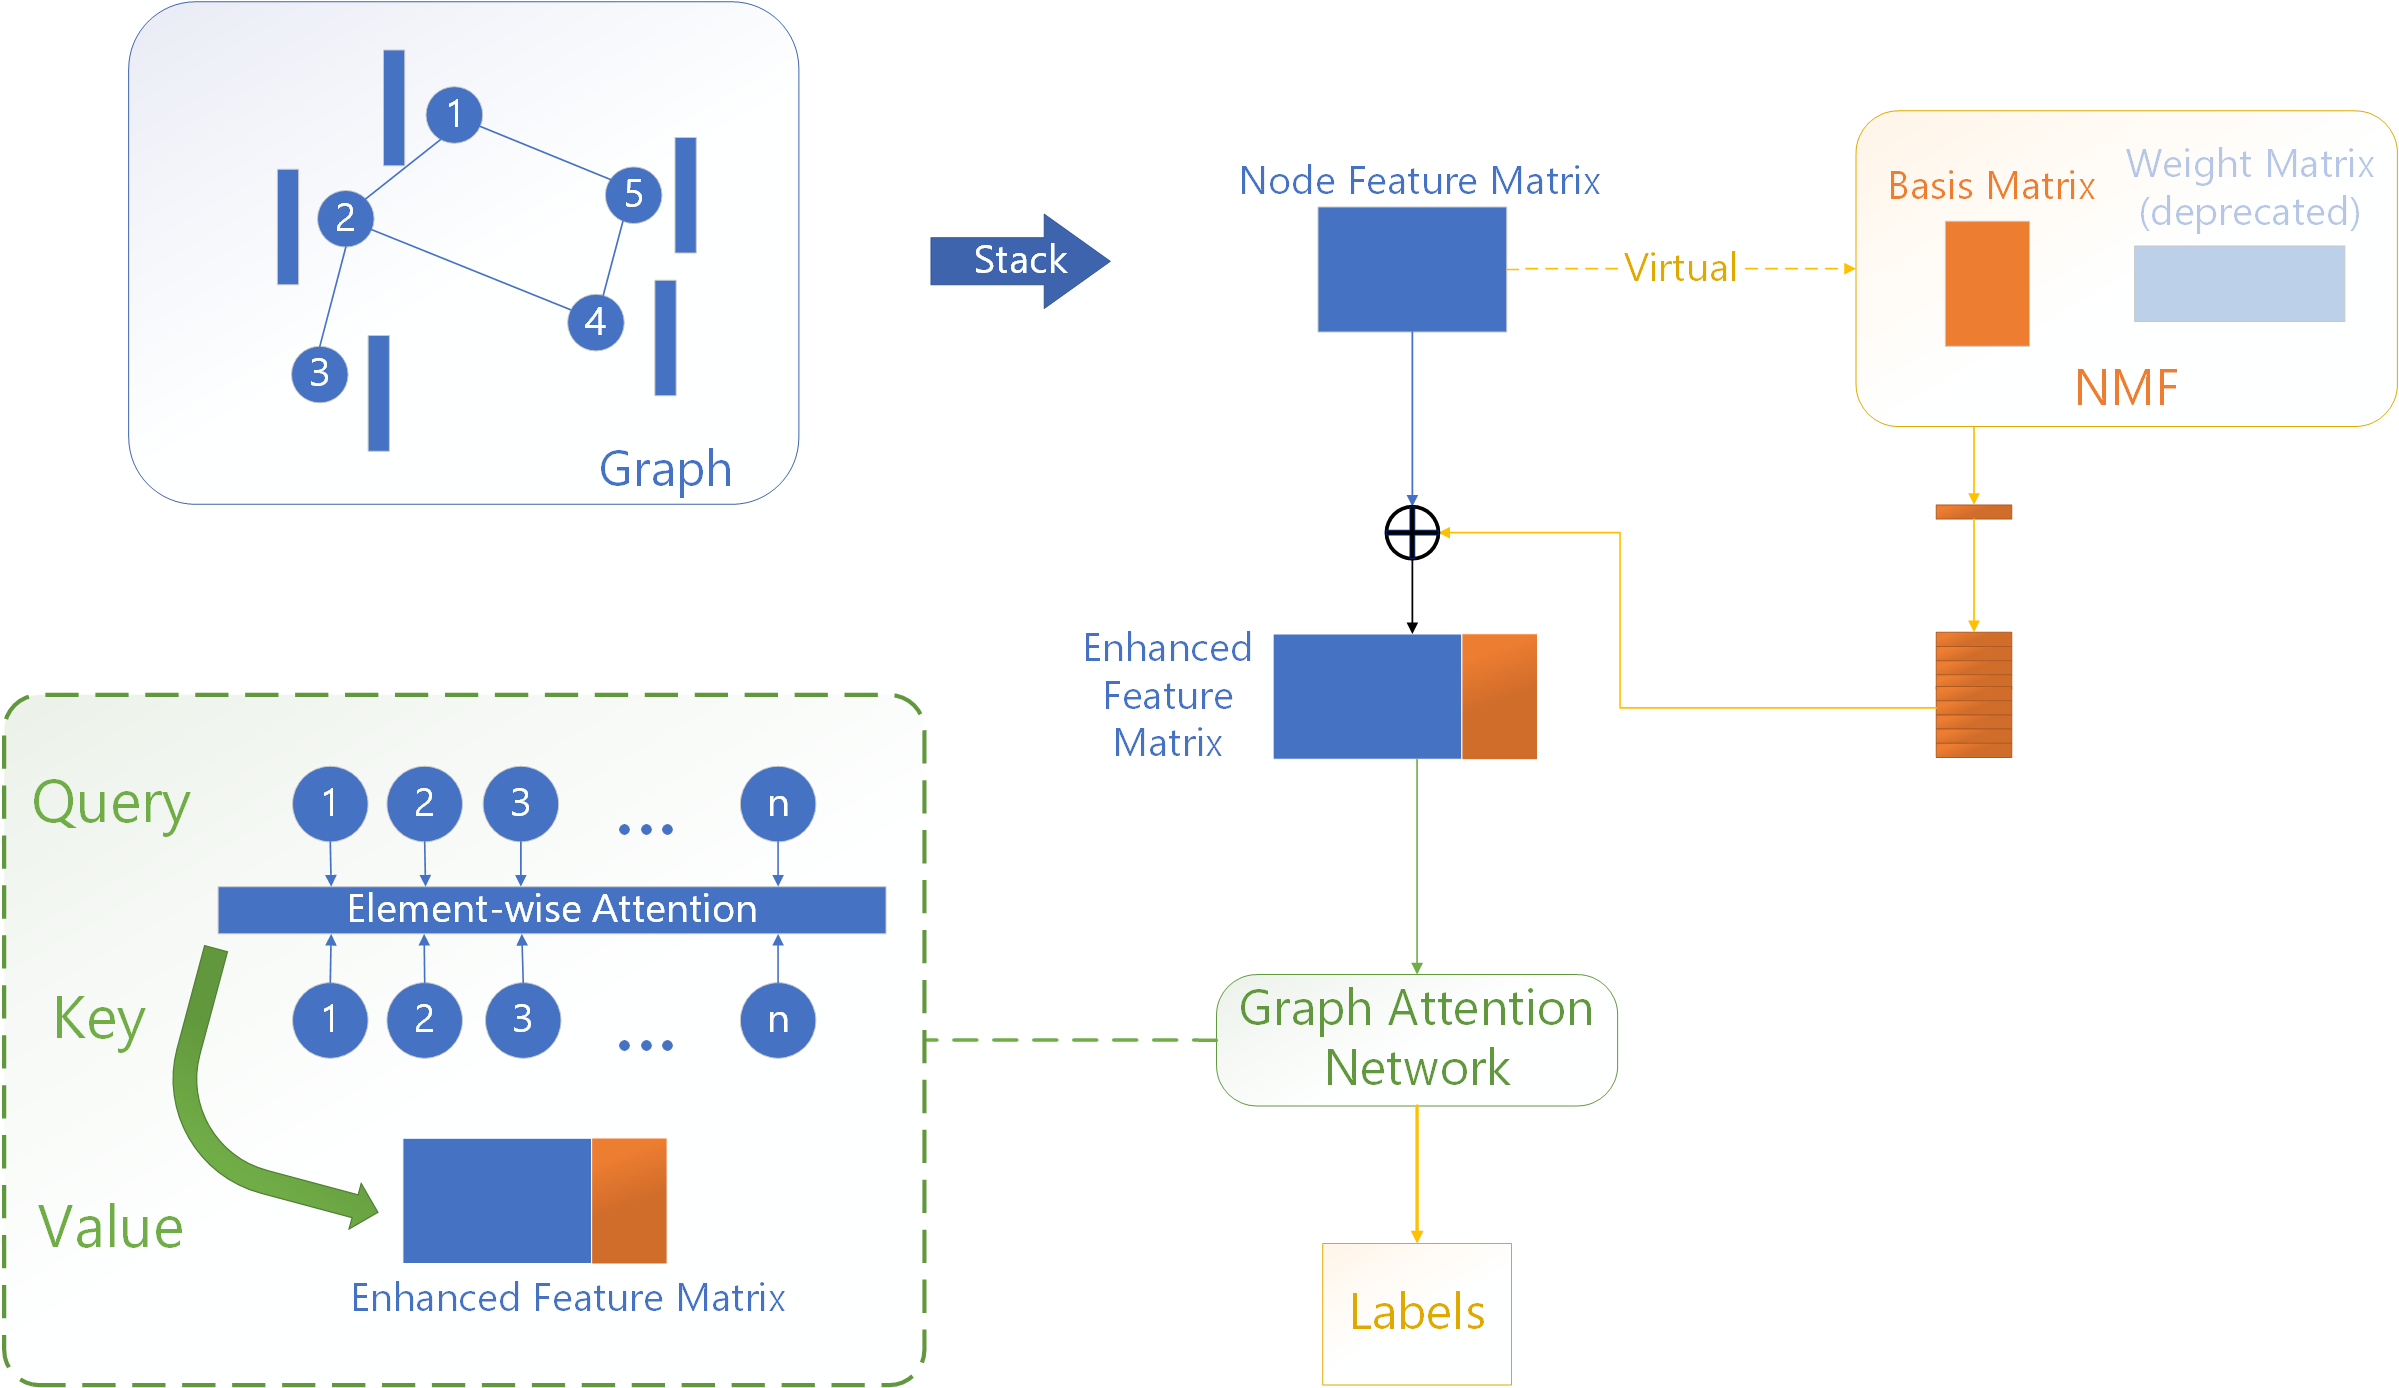
\includegraphics[width=\linewidth]{graph1}
	\caption{Illustrated general pipeline of NMF-GNN. Random initialized basis matrix is aggregated into a global feature vector and concatenated to each row of original feature matrix. Then the matrix is updated through message passing backbone, with parameters simultaneously optimized. }
	\label{fig:graph1}
\end{figure}
		
	\subsection{Pipeline}
	The general pipeline of our approach is shown in figure \ref{pipeline}.
	The original matrix of node features $ \mathbf{X}\in \mathbb{R}^{n\times m} $ is factorized as $ \bf X\approx WH $, where $ \mathbf{W}\in \mathbb{R}^{n\times k} $ and $ \mathbf{H}\in \mathbb{R}^{k\times m} $ represents the basis and combination matrix respectively, where $ k $ is manually defined. Then basis matrix $ \mathbf{W} $ is embedded into a feature vector $ \bf w $ by aggregation operations. In our implementation the aggregation is chosen as row-wise mean, which is $  \mathbf{w}=\frac{1}{N}\sum\limits_{i=1}^N \mathbf{W}_{i, :} $. These operation are all differentiable which can be optimized via backpropagation. 
	Then $ \bf w $ is concatenated with all node features $ \mathbf{v}_i,\. i\in [1,N] $ into the new vector $ \mathbf{v}'_i $, which is denoted as 
	\begin{equation}\label{key}
		\mathbf{v'}_i = \Bigg|\Bigg|\left\{\mathbf{v}_i, \mathbf{w}\right\}.
	\end{equation}
	Then the fused vectors are taken into the following message passing defined by GAT. GAT calculates self-attention inside the node set, which attention score calculated between weighted key vectors $ \mathbf{k}_i $ and query vectors $ \mathbf{q}_j $ in the node set, where the weight matrix $ \bf R $ is shared in the message passing. The process can be mathematically expressed as
	\begin{equation}\label{key}
		\mathbf{A} = \delta(\frac{\exp(\mathbf{R}\mathbf{Q} \mathbf{K}^\intercal\mathbf{R}^\intercal)}{\sqrt{m}})
	\end{equation}
	where $ \mathbf{A}_{ij} $ denotes the attention score between $ i $-th query vector and $ j $-th key vector, $ m $ denotes the feature dimension and $ \delta() $ denotes a nonlinear activation function (LeakyRELU in the original approach). Then the vector is updated through attention-weighted fusing of other node features, which is 
	\begin{equation}\label{key}
		\mathbf{H}^{(t+1)} = \sigma(\mathbf{AWH}^{(t)})
	\end{equation}
	where $ \sigma $ is a nonlinear function. 
	
	\section{Experiments}
	\subsection{Implementation details}
	\textbf{Model variants.}	There are 2 kinds of variants along the model
	
	\textbf{Baseline model.} Former illustration shows that our model can be easily plugged on any message passing frameworks. The baseline model is implemented using attention
	We basically implemented our model on GAT, with both multi-head attention layers and output attention aggregation layer. Furthermore, ablation studies are performed on partial-NMF and full-NMF conditions, which are NMF implemented on only output attention layer and output + multi-head attention layers correspondingly. Model configuration and training strategies are fixed along experiments to make a fair comparison. 
	
	
	\subsection{Implementation details}
	The framework is implemented by PyTorch 1.7.1 in Python 3.9 with CUDA 11.2 and executed on an NVIDIA \textregistered TESLA \textregistered V100 32GB GPU. 
	
	The result is shown in table \ref{tab:model}
	
%	\begin{center}
%		\begin{spacing}{1.1}
%			%longtable的意思是 这个表格可以跨页
%			\begin{longtable}{p{.1\textwidth}p{.7\textwidth}m{.3\textwidth}}
%				\caption{description}
%				\label{table1}
%				\toprule   %第一行线
%				%表示第一列占1.5cm 第二列占6cm 第三列占2cm 的距离 并且这几个字都是居中对齐
%				\multicolumn{1}{m{1.5cm}}{\centering Symbol} & \multicolumn{1}{m{6cm}}{\centering Definition} & \multicolumn{1}{m{2cm}}{ Unit} \\
%				\midrule   %第二行线
%				$V$ & index & -- \\
%				$X$ & The  & -- \\
%				$Y$ & The & -- \\
%				$Z$ & The  & -- \\
%				\bottomrule   %第三行线
%			\end{longtable}
%		\end{spacing}
%	\end{center}

%\begin{table}[htbp]   \caption{\label{tab:model}Comparison of validation performance of our model with GNNs on node prediction tasks (small scale). }   
%	\begin{tabular}{lcl}    
%		\toprule     & Cora & PubMed & OGB-ArXiv & OGB- \\    
%		\midrule   
%			GCN & 5 & 6 \\  
%			GAT & 8 & 9 \\  
%			GraphSAGE & & \\
%			GraphLSP & & \\
%			\hline
%			NMF-GNN-Partial + GAT &0.8000 & \\
%			NMF-GNN-Full + GAT & &\\
%		\bottomrule   
%	\end{tabular} 
% \end{table}
%
%\begin{table}[htbp]   \caption{\label{tab:backbone}Comparison of our model with different GNN backbones on node prediction tasks (small scale). }   
%	\begin{tabular}{lcl}    
%		\toprule     & Cora & PubMed & OGB-ArXiv & OGB- \\    
%		\midrule   
%		NMF-GNN-Partial + GCN & & \\
%		NMF-GNN-Full + GCN & &\\
%		NMF-GNN-Partial + GAT & & \\
%		NMF-GNN-Full + GAT & &\\
%		\bottomrule   
%	\end{tabular} 
%\end{table}



\begin{enumerate}
		\item 	Do the experiments on different datasets.
 \item 	We need to prove that NMF solution is not unique.
 \item 	If the solution is not unique, we should implement the multi-NMF to the GNN to capture different features.
\item 	Embed the NMF into the GAT network. NMF should share the parameters with GAT.
Besides, we need to test the deep NMF model to show whether the heretical NMF would have fine-grained topics.
\end{enumerate}
	
\begin{thebibliography}{00}
	\bibitem{b1} You, J., Ying, R., \& Leskovec, J. (2019). Position-aware graph neural networks. arXiv preprint arXiv:1906.04817.
	\bibitem{b2} Long, Q., Jin, Y., Song, G., Li, Y., \& Lin, W. (2020, August). Graph Structural-topic Neural Network. In Proceedings of the 26th ACM SIGKDD International Conference on Knowledge Discovery \& Data Mining (pp. 1065-1073).
	\bibitem{b3} Lee, D. D., \& Seung, H. S. (1999). Learning the parts of objects by non-negative matrix factorization. Nature, 401(6755), 788-791.
	\bibitem{b4} Feng, T., Li, S. Z., Shum, H. Y., \& Zhang, H. (2002, June). Local non-negative matrix factorization as a visual representation. In Proceedings 2nd International Conference on Development and Learning. ICDL 2002 (pp. 178-183). IEEE.
	\bibitem{b5} Huang, Z., Zhou, A., \& Zhang, G. (2012, October). Non-negative matrix factorization: A short survey on methods and applications. In International Symposium on Intelligence Computation and Applications (pp. 331-340). Springer, Berlin, Heidelberg.
	\bibitem{cora} Sen, P., Namata, G., Bilgic, M., Getoor, L., Galligher, B., \& Eliassi-Rad, T. (2008). Collective classification in network data. AI magazine, 29(3), 93-93.
	\bibitem{gat} Veličković, P., Cucurull, G., Casanova, A., Romero, A., Lio, P., \& Bengio, Y. (2017). Graph attention networks. arXiv preprint arXiv:1710.10903.
	\bibitem{gcn} Kipf, T. N., \& Welling, M. (2016). Semi-supervised classification with graph convolutional networks. arXiv preprint arXiv:1609.02907.
	\bibitem{nips} Lee, D. D., \& Seung, H. S. (2001). Algorithms for non-negative matrix factorization. In Advances in neural information processing systems (pp. 556-562).
	\bibitem{2} Trevisan, L. (2017). Lecture Notes on Graph Partitioning, Expanders and Spectral Methods. University of California, Berkeley, https://people. eecs. berkeley. edu/~ luca/books/expanders-2016. pdf.
	\bibitem{3} Hammond, D. K., Vandergheynst, P., \& Gribonval, R. (2011). Wavelets on graphs via spectral graph theory. Applied and Computational Harmonic Analysis, 30(2), 129-150.
\end{thebibliography}
	
\end{document}



